\setcounter{chapter}{2} 
\chapter{Theoretical background: Processes Implemented in the CTM3}\label{Chap:CTM3theory_ocean_hetReact}

Some of the processes that are implemented in the Oslo CTM3 requires some further explanation. Here, I will cover the theory behind the implementation of emissions of organic halogen species and the heterogeneous reaction surfaces.

\section{Oceanic emissions of halocarbons}\label{sec:oceanic_emissions}


The ocean is a natural source of gaseous halocarbons, and is therefore used here as a source needed for the bromine explosion to occur. Methyl halides ($\chem{CH_3X}$) and polyhagenated species ($\chem{CHBr_3}$, $\chem{CH_2Br_2}$) are released from the ocean, but methyl halides (particularly $\chem{CH_3Br}$) may also be emitted by biomass burning (\cite{SeinfeldSpyros}). 

\medskip

Bromoform ($\chem{CHBr_3}$) and dibromomethane ($\chem{CH_2Br_2}$) are used as the oceanic sources of bromine in this implementation. The anthropogenic signal of methyl halides are not taken into consideration in this thesis. Nor are the difference in lifetime ($\chem{CH_3Br} \sim$ 1 month, $\chem{CH_2Br_2} \sim$ 4 months) as well as seasonal variations. 


\medskip

Bromoform, $\chem{CH_3Br}$, is added as a source from the ocean based on the emission scenario suggested by \cite{Liang2010} (scenario A, Figure \ref{fig:Liang2010}). This scenario was chosen as it has latitudinal-dependent emission field covering the whole globe. The global emissions estimated by \cite{Liang2010}, scenario A, were 425 Ggyr$^{-1}$ of $\chem{CHBr_3}$ and 57 Ggyr$^{-1}$ of $\chem{CH_2Br_2}$, respectively.

\medskip

The thought behind the implementation (the variable \texttt{POLL\_CHBr3}) is that it contains the emissions from both $\chem{CHBr_3}$ and $\chem{CH_2Br_2}$. The reason for this is that there was already an organic halogen existing in the CTM3, methyl bromide ($\chem{CH_3Br}$), which would only be used by the model when the stratosphere was activated (which was not the case in my runs). Thus, this was used for the mapping of the concentration of $\chem{CHBr_3}$ and $\chem{CH_2Br_2}$ instead. To simplify this source further, $\chem{CH_2Br_2}$ was added to the emission scheme in Figure \ref{fig:Liang2010} by a scaling factor based on the global emissions. 

\medskip

The scaling factor was calculated by finding the yield of bromine from both $\chem{CHBr_3}$ and $\chem{CH_2Br_2}$ based on reactions \ref{R:10} and \ref{R:11}, and expressing this in terms of $\chem{CHBr_3}$. 

\begin{align*}
    \chem{X} & = 57 Gg \chem{CH_2Br_2}yr^{-1} \\
    \chem{Y} & = 425 Gg \chem{CHBr_3}yr^{-1} 
\end{align*}

The bromine yield, \chem{Z}, from Reactions \ref{R:10} and \ref{R:11} is then: 

\begin{align*}
    \chem{Z} & = \Big(3\cdot\Big(\frac{X}{M_{\chem{CH_2Br_2}}}\Big) + 2\cdot\Big(\frac{Y}{M_\chem{CHBr_3}}\Big)\Big)\cdot M_{\chem{Br}} \\
    & = \Big(3\cdot\Big(\frac{425 Gg \chem{CHBr_3}yr^{-1}}{252.73 g mol^{-1}}\Big) + 2\cdot\Big(\frac{57 Gg \chem{CH_2Br_2}yr^{-1}}{173.83 g mol^{-1}}\Big)\Big)\cdot79.90 g mol^{-1} \\
    & = 455 Gg\chem{Br}yr^{-1}
\end{align*}

The emission of $\chem{CHBr_3}$, had this been the only source of bromine, is expressed by $Y'$, which is: 

\begin{align*}
    \chem{Y'} & = \frac{1}{3}\cdot\frac{252.73 g mol^{-1}}{79.90 g mol^{-1}}\cdot455.49Gg\chem{Br}yr^{-1} \\
    & = 479.73 Gg \chem{CHBr_3}yr^{-1}
\end{align*}

This is used in the scaling factor, $f$:

\begin{equation*}
    f = \frac{\chem{Y'}}{Y} \approx 1.13
\end{equation*}


Emissions are then found according to their latitudinal band, and whether the grid box is located over ocean or the coast (for more information about the actual implementation, see Section \ref{sec:tropchem_oslo}). If the location is above 50 $^o$ North over ocean, for example, the emission is taken to be $0.05\times10^{-13}$ kgm$^{-2}$s$^{-1}\times k$. (The conversion to molecules cm$^{-3}$s$^{-1}$ can be seen in Section \ref{sec:tropchem_oslo}). 


\subsection{Emission inventory}

The emission inventory of $\chem{CHBr_3}$ and $\chem{CH_2Br_2}$ by \cite{Liang2010} was compared against observations and other emission inventories by \cite{Hossaini2013}. The results can be seen in Figures \ref{fig:Hosaini_fig5} and \ref{fig:Hosaini_fig6} in the Appendix. They show a reasonable agreement between the observations and mixing ratios suggested by \cite{Liang2010} for the stations \acrfull{alt}, \acrfull{brw} and Summit (SUM), which are of most relevance in this setting. The inventory, however is rather crude and simple as it does not take into account seasonality, extrapolar results of agreement with observations. 


\begin{figure}
    \centering
    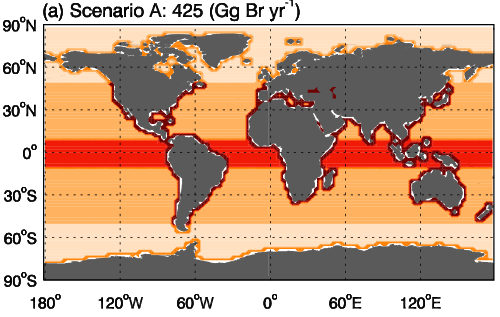
\includegraphics[width = 0.5\textwidth]{Chapter3_Theory_ocean_hetReact/images/liang_etal_2010.png}
    \caption{Global emission distribution of $\chem{CHBr_3}$. Scenario A is applied for the \chem{CHBr_3} with emissions taken as the half point of the colorbar. Image taken from \cite{Liang2010}}
    \label{fig:Liang2010}
\end{figure}



\section{Heterogeneous chemistry}\label{sec:het_chem}

Bimolecular reactions are reactions in which two chemical species react and produce a different set of species (\cite{Jacob1999}). The reaction can be written as: 

\begin{equation*}
    A + B \rightarrow C + D
\end{equation*}

The reaction rate, $k$, is the time rate of change of a concentration of the reactant in the reaction (\cite{AtmModFund}). It is given by: 

\begin{equation*}
    -\frac{d}{dt}[A] = -\frac{d}{dt}[B] = \frac{d}{dt}[C] = \frac{d}{dt}[D] = k[A][B]
\end{equation*}

in which the bracketed species $[]$ denotes the number densities (in this case the number of molecules per $cm^3$) and $k$ is the second-order deposition-rate constant for the reaction in $cm^3\text{molecule}^{-1}s^{-1}$. The product $[A][B]$ is proportional to the frequency of collisions. A bimolecular reaction could also be a self-reaction, in which $B = A$ and the reaction rate would be:

\begin{equation*}
    -\frac{d}{dt}[A] = -\frac{d}{dt}[A] = \frac{d}{dt}[C] = \frac{d}{dt}[D] = k[A]^2
\end{equation*}

\subsection{Heterogeneous reactions on aerosol surfaces (Reactions \ref{R:8} and \ref{R:13})}\label{sec:aerosol_react}

The implementation of the aerosol Reactions \ref{R:8} and \ref{R:9} is based on the method described by \cite{CAO} and \cite{schwartz1986}. An overview of the constants used can be found in Table \ref{tab:constants}.

\medskip

The production rate of $\chem{Br_2}$ molecules for Reaction \ref{R:8} is given as: 

\begin{equation*}
    \frac{d}{dt}[\chem{Br_2}] = -\frac{d}{dt}[\chem{HOBr}] = k[\chem{HOBr}]
\end{equation*}

which has the first-order reaction-rate constant: 

\begin{equation*}
    k = \big(\frac{a}{D_g} + \frac{4}{v_{therm}\gamma}\big)^{-1}\alpha_{eff}
    \label{eq:reaction_rate_const}
\end{equation*}

in which $a$ is the aerosol radius, $D_g$ is the molecular diffusivity in the gas-phase, and the ratio $a/D_g$ represents the molecular diffusion limit. Following \cite{CAO}, the values of these are $a = 0.45 \mu m$ and $D_g = 0.2 cm^2s^{-1}$. 

\medskip

$v_{therm}$ in Equation \ref{eq:reaction_rate_const} is the mean molecular speed of \chem{HOBr} given as $v_{them} = \sqrt{8RT/(\pi \chem{M_{HOBr}})}$ in which $R$ is the universal gas constant (units $[Latm/Kmol]$), $T$ is the absolute temperature (units $[K]$) and $\chem{M_{HOBr}}$ is the molas mass of \chem{HOBr} (units $[g/mol]$). 

\medskip

$\gamma$ is the uptake coefficient or reaction efficiency of \chem{HOBr} on sea salt aerosols, i.e. the probability that the reaction will occur (\cite{SeinfeldSpyros}).

\medskip

$\alpha_{eff}$ is the surface-volume coefficient, i.e. the ratio of the total aerosol surface area, $A_{\text{aerosol}}$, and the total volume, $V$ (units $[cm^2cm^{-3}]$).
 
\medskip

The production rate of $\chem{Br_2}$ in Reaction \ref{R:8} is limited by the absorption of \chem{HOBr} and \chem{HBr}/\chem{HCl} in the suspended aerosol particles (\cite{CAO}). \cite{Hanson1994} expressed the effective uptake coefficient on small drops as: 

\begin{equation}
    \frac{1}{\gamma} = \frac{1}{\alpha}+ \frac{v_{therm}}{4H^*RT\sqrt{k_{liq}^ID_{liq}}f(q)}
    \label{eq:upt_coeff}
\end{equation}

\medskip

$R$ is the universal gas constant, $T$ is the temperature.

\medskip

$D_{liq}$ is the liquid phase diffusion coefficient (proportionality factor implying that a mass of the substance diffuses through a unit surface in a unit time at a concentration gradient of unity). 

\medskip

in which $\alpha$ is the mass accommodation coefficient. This quantity describes the probability that a gas or vapour particle will stick upon collision with the surface of a particle, where $0\leq\alpha\leq1$ (\cite{SeinfeldSpyros}). Following \cite{CAO}, this will be taken as unity. 

\medskip

$H^*$ is the effective Henry's law constant for the species in question. The Henry's law coefficient, $H$, is a proportionality factor between the amount of dissolved gas and it's partial pressure in the gas phase (\cite{Sander2015}, see also Section \ref{sec:wet_dep_henrys_law}).  

$k_{liq}^I$ is the first-order liquid reaction rate constant for the species in question, calculated by: 

\begin{equation}
    k_{liq}^I = k_{liq}^{II}[\chem{X}]_{liq}= k_{liq}^{II}H^*_\chem{X}P_\chem{X}
\end{equation}

In which $H^*_\chem{X}$ is the effective Henry's law constant for the species and $P_\chem{X}$ is it's partial pressure.

\medskip

$f(q)$ is determined by: 

\begin{equation}
    f(q) = \coth{q} -\frac{1}{q} = \frac{1}{\tanh{q}} -\frac{1}{q}
\end{equation}

where $q = a\sqrt{\frac{k_{liq}^I}{D_{liq}}}$, is a dimensionless quantity called the diffuso-reactive parameter. This is used to calculate the uptake rates (\cite{Hanson1994}). 


\subsubsection{Heterogeneous reactions over snow and ice surfaces (Reactions \ref{R:7})}\label{sec:snow_ice_react}


The implementation of the heterogeneous reactions over snow/ice surfaces also follows the method by \cite{CAO}. 

\medskip

The change in concentration for Reactions \ref{R:7} can be given as: 

\begin{equation*}
    -\frac{d}{dt}[\chem{HOBr}] = k[\chem{HOBr}]
\end{equation*}

in which the deposition-rate constant, $k$, is: 

\begin{equation*}
    k = \frac{v_d}{L_{mix}}\beta
\end{equation*}

Thus, the deposition-rate constant depends on the deposition velocity, $v_d$, at the snow/ice surface, the height of the boundary layer, $L_{mix}$ and the reactive surface ratio coefficient, $\beta$. 

\medskip

The deposition velocity, $v_d = (r_a + r_b + r_c)^{-1}$, is dependent on three resistances which are: 

\begin{itemize}
    \item The aerodynamic resistance, $r_a$. This is the resistance of the turbulent transport to bring the gas from the atmosphere to the surface, approximated as: $1/(u\kappa^2)(\ln(z/z_0))^2$, where $u = 8 ms^{-1}$ is the wind speed, $\kappa = 0.4$ is the Von Karman constant, $z$ is the surface layer height, approximated as the lower $10\%$ of the boundary layer, i.e. $z = 0.1L_{mix}$, and $z_0$ is the surface roughness length which is approximated as $10^{-5} m$ for ice surfaces. $r_a$ is therefor dependent on local properties. 
    \item The quasi-laminar layer resistance, $r_b$, is the ability of molecular diffusion to transfer gas across a liquid-laminar layer above the surface. It is thus given as $r_b = z_0/D_g$
    \item The resistance due to the reaction loss, $r_c$ is given as $r_c = 4/v_{therm}\gamma$. The uptake coefficient is taken as $\gamma = 0.06$ including the assumption that the source of $\chem{H^+}$ and halogen ions are limitless at the snow/ice surface. 
\end{itemize}

$L_{mix}$ denotes the typical stable boundary layer height which may, in Polar regions, range from near-zero up to approximately 1000 m depending on. Consequently, the deposition velocities vary.

\medskip

$\beta$ is the ratio of the total reactive surface (induced by the structure of snow/ice surfaces) to a flat area. Thus, for a completely flat surface, $\beta$ equals 1. 

\begin{table}[ht]
\centering
\resizebox{\columnwidth}{!}{%
\begin{tabular}{|llll|}
\hline
\textbf{Variable} & \textbf{Quantity}    & \textbf{Unit}       & \textbf{Description}                                       \\ \hline
\multicolumn{4}{|c|}{\textbf{\chem{HOBr}}}                                                                 \\ \hline
$\alpha$          & $1.0$                & Dimensionless       & Mass accommodation coefficient                             \\
$\alpha_{eff}$    & $1.0 \times 10^{-6}$ & $cm^{-1}$           & Surface-volume coefficient                                 \\
$a$               & $0.45$               & $\mu m$             & Typical aerosol radius                                     \\
$\beta$           &                      & Dimensionless       & Ratio of the total reactive surface area to a flat surface \\
$D_{liq}$         & $5.0\times10^{-6}$   & $cm^2s^{-1}$        & Liquid phase diffusion coefficient                         \\
$D_g$             & $0.2$                & $cm^2s^{-1}$        & Molecular diffusivity                                      \\
$H^*$             & $1.7 \times10^4$     & $molL^{-1}atm^{-1}$ & Effective Henry's law constant                             \\
$M_{\chem{HOBr}}$ & $96.91\times10^{-3}$ & $kg mol^{-1}$       & Molar mass of \chem{HOBr}                 \\ \hline
\multicolumn{4}{|c|}{\textbf{\chem{HBr}}}                                                                  \\ \hline
$H^*$             & $3.0\times10^{8}$    & $molL^{-1}atm^{-1}$ & Effective Henry's law constant                             \\
$k_{liq}^{II}$    & $5.0\times10^{4}$    & $L mol^{-1}s^{-1}$  & Second order liquid rate reaction constant                 \\ \hline
\multicolumn{4}{|c|}{\textbf{\chem{HCl}}}                                                                  \\ \hline
$H^*$             & $3.0\times10^{6}$    & $molL^{-1}atm^{-1}$ & Effective Henry's law constant                             \\
$k_{liq}^{II}$    & $1.0\times10^{5}$    & $L mol^{-1}s^{-1}$  & Second order liquid rate reaction constant                 \\ \hline
\multicolumn{4}{|c|}{\textbf{$\chem{BrONO_2}$}}                                                                             \\ \hline
$\gamma$          & $0.06$               & Dimensionless       & Effective uptake coefficient                               \\ \hline
\end{tabular}
}
\caption{Overview of constants taken from \cite{CAO}}
\label{tab:constants}
\end{table}



\subsection{Photochemistry}

For photochemical reactions, the rate expression is (\cite{AtmModFund}):

\begin{equation*}
    A + hv \rightarrow B + C
\end{equation*}

and the rate expression is: 

\begin{equation*}
    \frac{d[A]}{dt} = -J[A]
\end{equation*}

In which $J$ is a first-order photolysis rate coefficient of species $A$ (units: $s^-1$). 

\section{Wet deposition and Henry's law}\label{sec:wet_dep_henrys_law}

Henry's law expresses the proportional relationship between the amount of gaseous and dissolved gas (\chem{A}) in equilibrium (\cite{SeinfeldSpyros}): 

\begin{equation*}
    \chem{A(g)} \rightleftharpoons \chem{A(aq)}
\end{equation*}

The proportionality factor is dependent on the partial pressure of \chem{A} in the gas phase and the dissolved \chem{A} such that: 

\begin{equation}
    [\chem{A(aq)}] = H_Ap_A
    \label{eq:Henryslaw}
\end{equation}

In which $H_A$ is the Henry's law coefficient and $p_A$ is the partial pressure of \chem{A(g)}. 

\medskip

In this context, and widely used by atmospheric chemists, the Henry solubility, $H^{cp}$ is applied (\cite{Sander2015}). Rearranging Equation \ref{eq:Henryslaw} gives: 

\begin{equation}
    H^{cp} \equiv \frac{C_A}{p_A}
    \label{eq:HenrySol}
\end{equation}

The temperature dependence of the Henry's law coefficient, which is an equilibrium constant, can be described by the van't Hoff equation (\cite{Sander2015} and references therein): 

\begin{equation*}
    \frac{d\ln(H)}{d(1/T)} = \frac{-\Delta_{sol}H}{R}
    \label{eq:vantHoff}
\end{equation*}

In which $\Delta_{sol}H$ is the change in enthalpy of dissolution ($H$ in this case does not refer to the Henry's law constant). $R$ is the universal gas constant. 


Hva er wet deposition? Hvordan relateres Henrys law til wet deposition?


The Henry's law constants can be seen in Section \ref{sec:scav_wet} in Table \ref{tab:Henrys_law}. 


\section{3-body reactions}


Reactions \ref{R:clono2} and \ref{R:13} were implemented by using the 3 body reaction scheme for their reaction rate constants. \cite{SovdeManual}. 

Smooth og grei!